% !TEX root = 0_main.tex

\section{Case Study: Amara On Demand}
\label{sec:case-study}

Amara is a project which sustains an open and collaborative platform for the creation of subtitles \cite{jansen_amara_2014}. Examples of organisations employing Amara's platform to create subtitles drawing on volunteer engagement include Khan Academy, Scientific American, and the California Academy of Science \cite{amara}. More specifically, our focus in this research is placed on the use of Amara's platform for the creation of subtitles as an on-demand and paid service: Amara On Demand (AOD). AOD was launched in 2013 \cite{zelickson2019} as a result of the success \cite{jansen_amara_2014} of Amara's platform (Figure \ref{fig:aod-platform} shows a screenshot of AOD's subtitling tool). AOD is organised as a non-profit organisation, under the umbrella of the Participatory Culture Foundation. AOD is inspired by cooperative and commoning practices \cite{gray2019ghost}, presenting a remarkable contrast when compared with the market-based logic of other crowdsourcing platforms. While AOD grew into its own enterprise within \textit{Amara.org}, it adopted the values of the original volunteer community \cite{amaraorg}. %Amara.org’s stated mission captures its commitment to open, collaborative creation that eliminates barriers to accessing online content \cite{amaraorg}.
%\begin{quote}
   % ``We are driven by our mission to foster a media ecosystem that enables everyone to benefit from online video content. Content that can enrich lives, but is not currently available to those who cannot hear or understand the language of the video. We believe a participatory and inclusive world leads to a more understanding and caring society.''
%\end{quote}


\begin{figure}[ht]
    \centering
    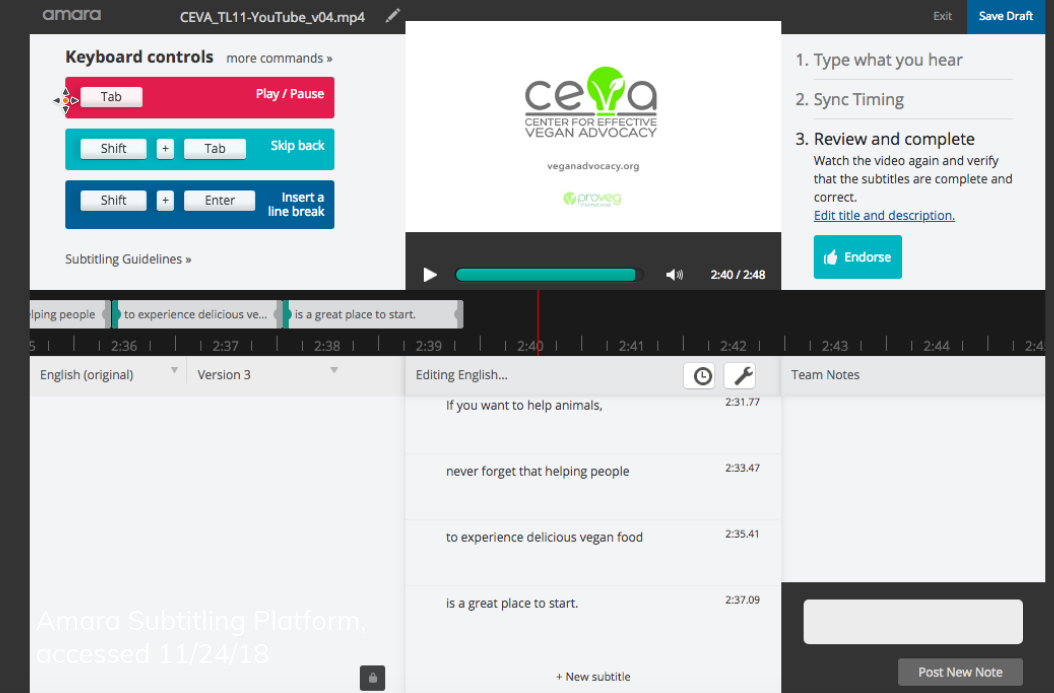
\includegraphics[width=\columnwidth]{figures/AOD_platform.png}
    \caption{Screenshot of AOD's subtitling platform, captured on 24th November 2018.}
    \label{fig:aod-platform}
\end{figure}

Over the past years, AOD moved from a few linguists to more than nine hundred at the time of writing\footnote{As self-reported by key members of AOD's core team during the interviews.} The work of linguists in AOD is remunerated and they are organised on a per-language direction basis and in which English operates as the master language. For example, if a customer requires a set of videos in German to be subtitled into Spanish, this will involve the groups German->English and English->Spanish. In order to join AOD, linguists are required to submit a resume, two examples of captioned or translated work, and pass an online interview as well as a test. The test is intended to ensure linguists understand AOD's guidelines, maintaining quality and thus, client satisfaction.

An essential part of AOD is the core team that facilitates and oversees the whole production process, coordinating and sustaining the infrastructure required for the successful creation of subtitles and captioning. The core team operates as a central node in AOD, although their members are globally distributed. The core team also monitors linguists' compliance with the rules. In AOD, there are explicit rules, practices, and guidelines to govern participation and foster professionalism. For linguists, this means completing tasks by deadlines, not assigning themselves more than one video ``at the same time'', and adhering to project-specific rules. Linguists are expected to adhere to them in order to receive payment.